\chapter{Hijerarhija ograničavajućih volumena (eng. Bounding volume hierarchy - BVH)}\label{cha:BVH}
S obzirom da su objekti u praksi vrlo komplicirani te sastavljeni od puno različitih primitiva, potrebna nam je struktura podataka koja će na vjeran način ograničiti naš objekt. Ukoliko objekt ograničimo manjim volumenima i te volumene posložimo u stablo, dobili smo određenu hijerarhiju volumena ili BVH. Stablo prikazujemo kao:
\begin{itemize}
	\item Root element stabla ograniči cijeli objekt
	\item Njegova djeca ograniče lijevu i desnu polovicu objekta
	\item Djeca od ta 2 elementa podijele taj volumen na 2 dijela itd.
	\item Listovi sadrže ograničavajući volumen najmanjeg primitiva ili sami primitiv
\end{itemize}
To prikazujemo ovako:
\newpage
\begin{figure}[!http]
		\begin{center}
			\includegraphics[height = 8 cm, width = 8 cm, keepaspectratio = true]{simple_bvh}
			\caption{Primjer BVH\cite{4}}
			\label{fig:6}
		\end{center}
\end{figure}
Konceptualno, objekt bi prikazujemo na takav način. Ograničavajući volumen koji je roditelj u stablu, ograničuje druga 2 volumena i tako sve do listova koji su primitivi. Nešto kompleksnija struktura bila prikazuje se ovako:
\begin{figure}[!http]
	\begin{center}
		\includegraphics[height = 8 cm, width = 8 cm, keepaspectratio = true]{complex_bvh}
		\caption{Prikaz kompliciranije BVH \cite{4}}
		\label{fig:7}
	\end{center}
	\end{figure}
BVH možemo izgraditi od bilo kojih ograničavajućih volumena. U konačnici izgradnja samog stabla je uvijek proporcionalna broju elemenata od kojih je objekt sastavljen (složenost O(n))\cite{1}. Ono što je u ovom slučaju najbitnije je to da stablo ne moramo graditi u svakom frameu što prilično ubrzava posao. Također, važno je da stablo bude balansirano. Ukoliko je stablo dobro balansirano, objekt koji ograničavamo će biti točnije ograničen, nego što bi to bilo u suprotnom slučaju. Za detektiranje sudara moramo samo provjeriti sudaraju li se u početku root elementi stabala. Ukoliko ne, odmah možemo prekinuti daljnju pretragu sudara, no sam algoritam i implementacija biti će prikazana kasnije.
	
Za potrebe ovog objekta odabrali smo AABB stablo zbog njegove efikasnosti i jednostavnosti prilikom implementacije. Kako je već i spomenuto, sudar između 2 AABB-a vrlo je jednostavno detektirati i to je glavna prednost ovoga stabla.

\section{AABB stablo}
AABB stablo možemo prikazati kao:
\begin{figure}[!http]
	\begin{center}
		\includegraphics[height = 8 cm, width = 8 cm, keepaspectratio = true]{AABB_tree}
		\caption{Prikaz kompliciranog AABB stabla \cite{5}}
		\label{fig:8}
	\end{center}
\end{figure}
Stablo sa slike \ref{fig:8} izgleda komplicirano. Ali, već i iz kompliciranog objekta možemo vidjeti da se događaju pogreške. Te pogreške s jedno strane ipak nisu toliko bitne jer kada dođemo do lista u stablu, nećemo detektirati sudar. Jednostavniji primjer AABB stabla izgledao bi ovako:
\begin{figure}[!http]
	\begin{center}
		\includegraphics[height = 8 cm, width = 8 cm, keepaspectratio = true]{simple_aabb_tree}
		\caption{Prikaz jednostavnog AABB stabla}
		\label{fig:9}
	\end{center}
\end{figure}
\newline
Ovdje smo cijelu scenu podijelili AABB stablom, ali pristup je isti dijelimo li cijelu scenu ili jedan objekt. Scenu ćemo podijeliti ukoliko želimo provjeriti sudar zrake sa određenim objektom, a objekte ćemo podijeliti ukoliko želimo provjeriti sudar između samih objekata \cite{1}. 
\subsection{Ograničavanje 2 AABB minimalnim volumenom}\label{subsec:combineAABB}
Prije nego izgradnje AABB stabla, potrebno je pronaći način kako 2 AABB ograničiti jednim većim volumenom. Uvjet je da je taj ograničavajući volumen minimalan za 2 AABB čiji ograničavajući volumen tražimo.

\begin{figure}[!http]
	\begin{center}
		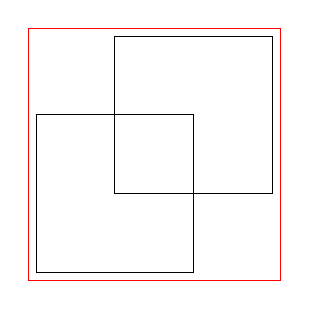
\begin{tikzpicture}
			\draw  (-2,-2) rectangle (0,0);
			\draw (-1,-1) rectangle (1,1);
			\draw[red] (-2.1,-2.1) rectangle (1.1,1.1);
		\end{tikzpicture}
		\label{fig:10}
		\caption{Minimalni ograničavajući volumen označen crvenom bojom}
	\end{center}
\end{figure}

Kako je to spomenuto ranije u poglavlju \ref{sec::AABB_representation}, koristili smo reprezentaciju AABB-a sa točkom centra i radijusom. Pronalaženje ograničavajućeg volumena za ovakvu reprezentaciju AABB-a malo je zahtjevnije nego u slučaju sa min-max reprezentacijom.
\begin{algorithm}
\caption{Algoritam za izračunavanje minimalnog ograničavajućeg volumena za 2 AABB-a}
\label{alg:fatten_aabb}
\begin{algorithmic}
	\Function {getFattenAABB}{$AABB$ $a$, $AABB$ $b$}
		\State $AABB FattenAABB$ 
		\State$FattenAABB.r =\frac{distance(a.center,b.center)}{2}\ + Max(a.r,b.r)$
		\State$FattenAABB.center = median(a.center,b.center)$
		\State \Return $FattenAABB$
	
	\EndFunction
\end{algorithmic}
\end{algorithm}
\newline
Jednostavnom matematikom izračunamo udaljenost između 2 centra i pribrojimo joj veći od 2 radijusa (u našem slučaju radijusi su jednaki, ali zbog svih slučajeva stavljen je odabir maksimuma) da dobijemo radijus za naš AABB. Centar je jednostavno određen srednjom točkom između 2 centra od ulaznih AABB-a. Veći radijus odabran je iz razloga da s manjim nećemo moći ograničiti oba AABB-a i to zapravo neće biti ograničavajući volumen za 2 željena AABB-a. 
\subsection{Izgradnja AABB stabla}

Za izgradnju AABB stabla postoje 3 načina\cite{3}: 
\begin{itemize}
	\item \emph{Top down} konstrukcija
	\item \emph{Bottom up} konstrukcija
	\item Dodavanje elemenata u stablo
\end{itemize}
Za sva 3 načina, potrebno je odabrati strategiju koja će napraviti što manje stablo. Ukoliko nam je stablo veliko pretraga elemenata u kojima se događa sudar će duže trajati. Zbog toga, potrebno je odabrati strategiju koja će stvoriti dobro balansirano ili približno dobro balansirano stablo\cite{1}. Ukoliko i ne stvorimo dobru strategiju za izgradnju stabla, uvijek možemo balansirati stablo "ručno" tj. putem funkcije. Ovo nikako nije poželjan slučaj. Time se gubi dodatno vrijeme na procesoru i funkcija za balansiranje je sama po sebi komplicirana i zahtjeva O(n) operacija. Za \emph{Top down} i \emph{Bottom up} konstrukciju potrebno je odabrati ravninu presijecanja (eng. Partitioning plane). Izgradnja ovoga stabla je u principu kao izgradnja svakog drugog stabla, samo je odabir ravnine presijecanja posao koji zahtjeva veliku količinu znanja i testiranja da u konačnici naše stablo bude minimalno. 
Ravnina presijecanja, kao što joj i samo ime govori, presjeći će listu naših objekata i pripadajućih AABB-a na onaj način kojim ćemo dobiti što manje stablo.Najjednostavniji model ravnine presijecanja je taj da se u listi elemenata odabere median element i da s obzirom na njegov AABB, izrađuje lijeva i desna grana stabla. Kao što je već rečeno, root element stabla će biti cijeli objekt te je potrebno samo odabrati pripadajuću točko centra i radijus (na ranije spomenuti način opisan u poglavlju \ref{subsec:combineAABB} samo sa listom elemenata).

U ovom radu, odabrali smo treću strategiju za izgradnju stabla. Ubacivanje elemenata u prvom trenutku činilo se kao najlogičniji izbor jer je glavna ideja bila da se stablo elemenata izgrada prilikom sudara kuglica.

\begin{figure}[!http]
	\begin{center}

		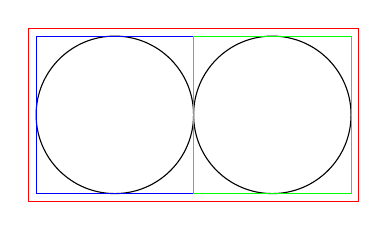
\begin{tikzpicture}
		\draw  (-1,0) circle (1);
		\draw (1,0) circle (1);
		\draw[blue] (-2,1) rectangle (0,-1);
		\draw[green] (0,-1) rectangle (2,1);
		\draw [red] (-2.1,1.1) rectangle (2.1,-1.1);
		\end{tikzpicture}
		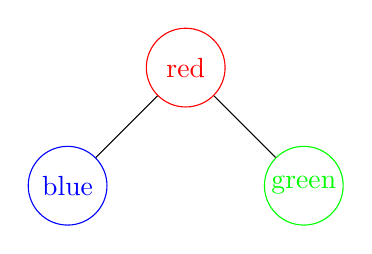
\begin{tikzpicture}[level distance=1.5cm,
		level 1/.style={sibling distance=3cm},
		level 2/.style={sibling distance=1.5cm}]
		\node[draw, circle,inner sep=1pt,minimum size = 1cm,red] {red}
		child {node[draw, circle,inner sep=1pt, minimum size = 1cm,blue] {blue}}
		child {node[draw, circle,inner sep=1pt,minimum size =1cm,green] {green}};
		\end{tikzpicture}		
	\end{center}
	\caption {Prikaz sudara 2 kuglice i pripadajućeg AABB stabla}
	\label{fig:11}
\end{figure}
Prema slici \ref{fig:11} stablo bi izgradili vrlo jednostavno. Nakon detekcije sudara, stvorili bi novi element, koji bi bio root element stabla (na slici \ref{fig:11} crvenom bojom). Njegov lijevi element pokazivao bi na lijevi AABB (plavom bojom), a desno dijete bi pokazivalo na desni AABB (zelenom bojom). 

Iako je primjer dosta trivijalan, još uvijek ne znamo kako nam klasa za AABB stablo izgleda, stoga još uvijek je sve prilično apstraktno. Klasa će sadržavati pokazivač na lijevi i desni element stabla. To smo riješili pomoću "pametnih" pokazivača tj. u C++-u, \texttt{unique\char`_ptr}. Ovakav tip pokazivača nas rasterećuje brige o memoriji i njezinom brisanju. Osim toga, sadržimo "običan" pokazivač na element roditelja. Važan podatak koji nam također treba je i dubina stabla. Osim svega navedenog, ovakav tip stabla gradili smo u konstrukturu. Nema smisla stvarati AABB stablo od jedne kuglice, stoga je ovo bio dobar način da se olakša sama implementacija algoritma za dodavanje dodatnih elemenata. Jednom kada bi izgradili stablo od 2 elementa, mogli smo dodati u njega bilo koji drugi element ubacivanjem na najbolju poziciju, tj. na poziciju gdje ćemo imati minimalno stablo.

\begin{lstlisting}[style=myC++, label = {code:8}, caption = {Implementacija klase za AABB stablo}]
class Node {
	typedef std::unique_ptr<Node> ptr;
	public:
		Node() = default;
		Node(const AABB_box bbox);
		Node(ptr &left, ptr &right);
	private:
		AABB_box box;
		ptr left;
		ptr right;
		Node *parent;
		int height;
};
\end{lstlisting}

Razmotrimo sljedeću situaciju:

\begin{figure}[!http]
	\begin{center}
		
		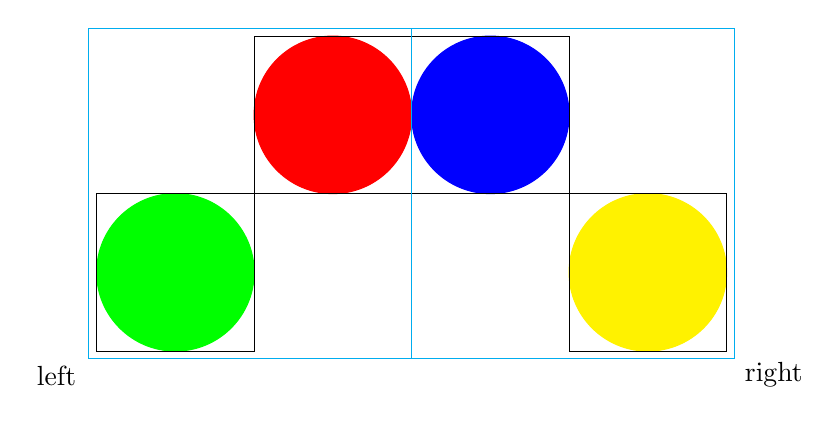
\begin{tikzpicture}
		\draw[red, fill = red]  (-1,0) circle (1);
		\draw[blue, fill = blue] (1,0) circle (1);
		\draw[green, fill = green] (-3,-2) circle (1);
		\draw[yellow, fill = yellow] (3,-2) circle (1);
		\draw (-2,1) rectangle (0,-1);
		\draw (2,1) rectangle (0,-1);
		\draw (-2,-1) rectangle (-4,-3);
		\draw (2,-1) rectangle (4,-3);
		\draw[cyan] (-4.1,-3.1) rectangle (4.1,1.1) node[black, pos = -.05] {left};
		\draw[cyan] (0,1.1) -- (0, -3.1) node[black, xshift = 4.6cm, yshift = -0.2cm] {right};
		\end{tikzpicture}
		\newline
	\end{center}
	\caption {Stablo od 4 kuglice}
	\label{fig:12}
\end{figure}
Prvo se sudare plava i crvena kuglica te se na taj način preko konstruktora izradi stablo sa 2 elementa. Nakon toga prvo udara žuta, a nakon toga zelena kuglica. Stablo koje ćemo dobiti izgledati će:
\newpage
\begin{figure}[!http]
	\begin{center}
		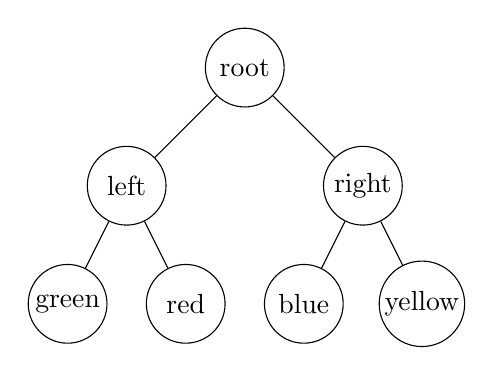
\begin{tikzpicture}[level distance=1.5cm,
		level 1/.style={sibling distance=3cm},
		level 2/.style={sibling distance=1.5cm}]
		\node[draw, circle,inner sep=1pt, minimum size = 1cm] {root}
		child {node[draw, circle,inner sep=1pt, minimum size = 1cm] {left}
			child {node[draw, circle,inner sep=1pt, minimum size = 1cm] {green}}
			child {node[draw, circle,inner sep=1pt, minimum size = 1cm] {red}}
		}
		child {node[draw, circle,inner sep=1pt, minimum size = 1cm] {right}
			child {node[draw, circle,inner sep=1pt, minimum size = 1cm] {blue}}
			child {node[draw, circle,inner sep=1pt, minimum size = 1cm] {yellow}}
		};

		\end{tikzpicture}
	\end{center}
	\caption {Prikaz AABB stabla za sliku \ref{fig:12}}
	\label{fig:12-1}
\end{figure}
Nakon udara svake kuglice, ubacujemo novi AABB u naše stablo. Za to je korišten vrlo jednostavan algoritam. Primjećujemo da svaki element koji ubacujemo u stablo će biti list, stoga možemo slobodno reći da ova funkcija realizira ubacivanje lista u stablo\cite{6}. Prije samog algoritma, treba naglasiti da napisani algoritam možda nije najtočniji i možda ne radi za sve slučajeve. Algoritam je u svakom slučaju nedovoljno testiran, ali za ovako mali primjer poslužio nam je da vrlo dobro prikažemo strukturu AABB stabla. Algoritam radi na jednostavan način. Iteriramo po kreiranom stablu i izračunavamo površinu AABB-a od elementa koji želimo ubaciti i lijevog i desnog djeteta. Ukoliko je površina AABB-a od lijevog djeteta i elementa manja od površine AABB-a i desnog djeteta, iteriramo u lijevu stranu stabla. Ako je obrnuto, iteriramo na desnu stranu i tako sve dok ne dođemo do posljednjeg elementa stabla\cite{6}. S obzirom jesmo li išli lijevo ili desno, tu ubacujemo naš novokreirani element u stablo. U zadnjem koraku, vraćamo se od lista prema root elementu i radimo "update" AABB-a nad svakim elementom stabla.\newpage
\begin{algorithm}
	\caption{Algoritam za ubacivanje lista u AABB stablo}
	\label{alg:leaf_insertion}
	\begin{algorithmic}
		\Function {insertLeaf}{$AABBtree$ $node$, $AABB$ $box$}
		\While {$node$ is not leaf}
		\If{$Surface(node->left->box,box)>Surface(node->right->box,box)$}
		 \State $isLeft = false$
		\State $node = node->right$
		\Else
		\State $isLeft = true$
		\State $node = node->left$
		\EndIf
		\EndWhile
		\If{$isLeft is true$}
		\State $NewNode(box)$
		\State $FatAABB(node->parent->left, box)$
		\State $NewNode->parent = node->parent$
		\State $node->parent->left = NewNode$
		\Else
		\State $NewNode(box)$
		\State $FatAABB(node->parent->right, box)$
		\State $NewNode->parent = node->parent$
		\State $node->parent->right = NewNode$
		\EndIf
		\State Update tree until root with new leaf
		\EndFunction
	\end{algorithmic}
\end{algorithm}\newpage

\subsection{Pronalaženje sudara između dva stabla}
Nakon što smo izgradili stabla detektirati sudar između više stabala trivijalna je stvar. S obzirom da su stabla sagrađena od AABB-a potrebno je provjeriti samo $root$ elemente, i ako se oni sudaraju idemo u daljnju elemenata stabala. Ukoliko sudara između $root$ elemenata nije detektiran, sudar se nije ni dogodio. Ovakav način zahtjeva O(logN) operacija \cite{1}. Za jednostavan primjer možemo promotriti situaciju sa 2 jednostavna stabla koja imaju po 2 elementa. 

\begin{figure}[!http]	
	\begin{center}
		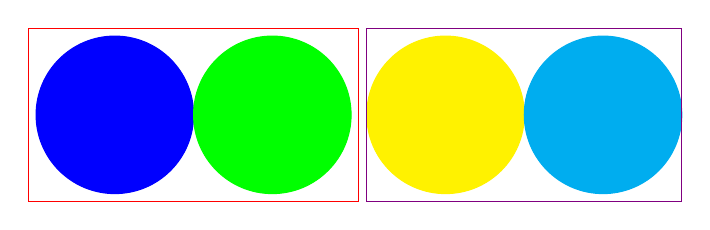
\begin{tikzpicture}
		\draw[fill = blue, blue] (-1,0) circle (1);
		\draw[fill = green, green] (1,0) circle (1);
		\draw[red] (-2.1,1.1) rectangle (2.1,-1.1);
		\draw[fill = yellow, yellow]  (3.2,0) circle (1);
		\draw[fill = cyan, cyan]  (5.2,0) circle (1);
		\draw [violet] (2.2,1.1) rectangle (6.2,-1.1);
		\end{tikzpicture}
	\end{center}
	\caption{Sudar između 2 jednostavna stabla}
	\label{fig:13}
\end{figure}
Za jedno i drugo stablo vrijedi struktura:
\begin{figure}[!http]	
	\begin{center}
		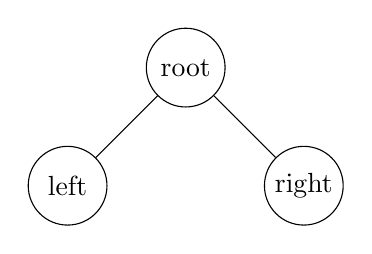
\begin{tikzpicture}[level distance=1.5cm,level 1/.style={sibling distance=3cm},level 2/.style={sibling distance=1.5cm}]
			\node[draw, circle,inner sep=1pt,minimum size = 1cm] {root}
				child {node[draw, circle,inner sep=1pt, minimum size = 1cm] {left}}
				child {node[draw, circle,inner sep=1pt,minimum size =1cm] {right}};
\end{tikzpicture}
	\end{center}
	\caption{Struktura stabla za sliku \ref{fig:13}}
	\label{fig:13-1}
\end{figure}
U nekom trenutku, mi želimo točno znati da se dogodio sudar između zelene i žute kuglice (kuglice su prikazane drugom bojom samo radi razumjevanja). Na već opisani način detektiramo na kojem mjestu će se dogoditi sudar. Kada otkrijemo u kojem se listu dogodio sudar, taj sudar ćemo na neki određeni način riješiti i napraviti update na cijelom stablu. U našem slučaju kuglice su se odbile bez gubitka energije.\newpage
\begin{algorithm}
	\caption{Algoritam za detektciju sudara između 2 AABB stabla}
	\label{alg:search_collision}
	\begin{algorithmic}
		\Function {searchCollision}{$AABBtree$ $a$, $AABBtree$ $b$}
		\If{$isCollision(a,b)$ is false}
		\Return
		\EndIf
		\While{$a$ is not leaf}
		\If{$isCollision(a->left,b)$}
		\State $a = a->left$
		\Else 
		\State $a = a->right$
		\EndIf	
		\EndWhile
		\While{$b$ is not leaf}
		\If{$isCollision(b->left,a)$}
		\State $b = b->left$
		\Else 
		\State $b = b->right$
		\EndIf	
		\EndWhile
		\State $ResolveCollision(a,b)$
		\EndFunction
	\end{algorithmic}
\end{algorithm}\
Kao i u algoritmu \ref{alg:leaf_insertion}, ovaj algoritam također nije istestiran do kraja i vjerovatno u sebi ima neke pogreške, no za ovako jednostavne primjere će raditi. Ovime smo zapravo pokazali da nakon potpunog razumijevanja AABB stabla i strukture možemo vrlo jednostavno napisati kod za izgradnju stabla i detektiranje sudara između 2 ili više stabala.
\newpage

\section{Prednosti i mane BVH-a}
Glavna prednost BVH-a je brzina izgradnje stabala. Ovakvim jednostavnim algoritmima možemo izgraditi stablo i u njemu vrlo brzo provjeriti sudare. Ukoliko imamo puno manjih objekata koji se kreću po sceni, pretraga sudara je vrlo brza. Stablo ne moramo raditi u svakoj sekundi, nego ga je dovoljno izgraditi na početku i zatim samo tokom vremena raditi "update". Nažalost, u prvoj fazi izrade projekta, nije se smislila adekvatna strategija za detektiranje sudara pa je i samo korištenja BVH-a palo u vodu. 

Mana BVH-a je što se vrlo dobro mora razumjeti struktura s kojom se barata. Za razliku od algoritama koji particioniraju prostor i koji su intuitivniji za shvatiti, BVH zahtjeva od nas da dobro razumijemo algoritam i da na pametan način odaberemo os po kojoj ćemo podijeliti objekt ili scenu. 

Zaključno, BVH je struktura podataka kojom ćemo na vrlo jednostavan i jeftin način detektirati sudare na sceni ili među objektima. Uz malo više uloženog vremena, možemo napisati vrlo dobar algoritam koji će vrlo brzo detektirati sve sudare na sceni. Kako je i rečeno, od ovoga se odustalo. S vremenom nakon što je i sama struktura postala jasnija, donijele su se neke druge odluke vezane za sam rad i više nije imalo smisla koristiti i dalje implementirati BVH.

 	
	